%\documentclass[handout]{beamer}
\documentclass{beamer}

\usepackage{bsymb}
\usepackage{b}
\usepackage{xcolor}

% Purpose of modelling?

% difference between axioms and invariants?
% can macine have axioms and vice versa

% why state invariants explicitly
% explain keywords

% ctr := ctr-1  versus  ctr=ctr-1

% explain skip

\mode<presentation>
{
    	%\usetheme{Warsaw}
	\setbeamertemplate{footline}
	{\centerline{\insertframenumber/\inserttotalframenumber}}
} 


\title{More on Event-B: Functions}

\author{\copyright\ Michael Butler}

\institute{ University of Southampton }



\begin{document}



\begin{frame}

\titlepage

\end{frame}














\begin{frame}

\frametitle{Partial Functions}

Special kind of relation:
each domain element has \alert{at most one range element }associated with
it. 

~

To declare $f$ as a partial function:
\[
     \mbox{\fbox{$~f ~\in~ X\pfun Y~$}}
\]

This says that $f$ is a \alert{many-to-one} relation

~

Each domain element is mapped to  \alert{one} range element:
\begin{eqnarray*}
    x~\in~ dom(f) ~
    &~~\implies~~& card(~f[\set{x}]~) ~=~ 1
\end{eqnarray*}

More usually formalised as a \alert{uniqueness} constraint
\begin{eqnarray*}
    x\mapsto y_{1}~\in~ f ~~\land~~ x\mapsto y_{2}~\in~ f
    &~~\implies~~& y_{1} = y_{2}
\end{eqnarray*}

\end{frame}



\begin{frame}


\frametitle{Function Application}

We can use \alert{function application} for partial functions.

~


If $x\in \dom(f)$, then we write ~~~\fbox{$f(x)$}~~~ for the
\alert{unique} range element associated with $x$ in $f$.

~

If $~x\not\in\dom(f)~$, then $f(x)$ is \alert{undefined}.

~

If $~card(~f[\set{x}]~)>1~$, then $f(x)$ is \alert{undefined}.

\end{frame}




\begin{frame}

\frametitle{Examples}

\[
\begin{array}{rcl}
    dir1 & = &
    \set{~  mary \mapsto 398620, \\
&&  ~~jim \mapsto 493028, \\
&&  ~~jane \mapsto 493028 ~}
\end{array}
~~~~~~
\begin{array}{rcl}
    dir2 & = &
    \set{~ mary \mapsto 287573, \\
&&  ~~mary \mapsto 398620, \\
&&  ~~jane \mapsto 493028 ~}
\end{array}
\]

Types of $dir1, dir2$ ? \hspace{0.3cm} $dir1(jim)$ ? \hspace{0.3cm} 
$dir1(sarah)$ ? \hspace{0.3cm} $dir2(mary)$ ? 
~
\pause
~
\vspace{0.5cm}
\begin{description}  \setlength{\itemsep}{4pt}
\centering \item    $dir1 ~\in~ Person \pfun Phone$
\item $dir2 ~\not\in~ Person \pfun Phone$
\pause
 \item $dir1(jim) ~=~ 493028$ 
\item  $dir1(sarah)$ ~is undefined 
\item $dir2(mary)$ is undefined
\end{description}


\end{frame}






\begin{frame}

\frametitle{Well-definedness and application definitions}

\begin{center}
\begin{tabular}{|c|c|}
\hline
Expression & Well-definedness condition \\[2pt] \hline
~&\\
$~~ f(x) ~~$ &  $~~x\in dom(f) ~\land~  f\in X \pfun Y ~~$  \\
~&\\ \hline\end{tabular}
\end{center}

~

The following definition of function application assumes that $f(x)$ is well-defined:

\begin{center}
\begin{tabular}{|c|c|}
\hline
Predicate & Definition \\[2pt] \hline
~&\\
$~~y = f(x) ~~$ &  $~x \mapsto y \in f~$  \\
~&\\ \hline\end{tabular}
\end{center}


\end{frame}





\begin{frame}

\frametitle{Function Operators}

All the \alert{relational operators} can be used on  functions
(restriction, subtraction, image, composition, etc).

~

Be \alert{careful} with some operators!

~

Suppose that $f$ and $g$ are functions.

\begin{itemize}
\item Set Union:~ $f \cup g$ is a  function provided
\[
    x\in \dom(f) ~\land~ x\in \dom(g) ~~~\implies~~~ f(x) = g(x)
\]
Why?


\item Inverse:~ $f^{-1}$ is not always a  function. Why
not?

\item What about $f;g$ ? 
\end{itemize}


\end{frame}




\begin{frame}


\frametitle{Function Overriding}

 \alert{Override} $f$ by $g$ ~~\fbox{~$f\ovl g$~}

~

 $f$ and $g$ must be partial functions of the \alert{same type}

~

Override: \alert{replace}  existing mappings with new ones


%
\begin{eqnarray*}
    dir1 & = &
    \set{~  mary \mapsto 398620, ~  john \mapsto 829483, \\
&& ~~~ jim \mapsto 493028, ~  jane \mapsto 493028 ~}
\end{eqnarray*}
\begin{eqnarray*}
dir1  \ovl   \set{~  mary \mapsto 674321 }  &=& ? \\ &\\
dir1  \ovl   \set{~  mary \mapsto 674321,~  jane \mapsto 829483 }  &=& ? \\\end{eqnarray*}

\end{frame}



\begin{frame}

\frametitle{Function Overriding Definition}

Definition in terms of function \alert{override} and \alert{set union}:

\pause
\begin{eqnarray*}
     f \ovl \set{a \mapsto b} &=&
     (\set{a}\domsub f) \cup \set{a \mapsto b} \\ &\\
     f \ovl g &=&
     (\dom(g)\domsub f) \cup g
\end{eqnarray*}
\end{frame}



\begin{frame}


\frametitle{Birthday Book Example}

Birthday book relates people to their birthday.

~

Each person can have at most one birthday.

~

People can share birthdays.

~

\setsA{
     PERSON ~~~  DATE
}

~

\variablesA{birthday}
%
\invariantA{
        birthday ~\in~ PERSON \pfun DATE   }

~

\initialisationA{
    birthday ~:=~ \set{} }

\end{frame}




\begin{frame}

\frametitle{Adding and checking birthdays}

~

\textit{Add} an entry to the directory: 
\pause
\operA{AddEntry}{
    \anyB{p,d}{p \in Person \\ 
						p\not\in dom(birthday)\\
		d\in Date}{birthday ~\assign~ birthday \cup \set{p\mapsto d}  }
    }

~

\alert{Check} a person's birthday:
\pause
\operA{Check}{
    \anyBs{p,d!}{ p\in dom(birthday) \\ d! = birthday(p)  }
    }


\end{frame}



\begin{frame}

\frametitle{Modifying a birthday}

\alert{Modify} an entry in the directory: 
\pause
\operA{ModifyEntry}{
    \anyB{p,d}{p \in dom(birthday) \\ d\in Date}{birthday ~\assign~ birthday \ovl \set{p\mapsto d}  }
    }

\alert{Syntactic shorthand:} \operA{ModifyEntry}{
    \anyB{p,d}{p \in Person \\ d\in Date}{ \alert{birthday(p) ~\assign~ d}  }
    }


\end{frame}





\begin{frame}


\frametitle{Function inverse}

Check birthdays on a particular date:
\operA{Who}{
    \anyBs{d,ps!}{d \in Date  \\ ps! = birthday^{-1}(d)  }
    }


\begin{itemize}
\item Is this mathematically valid? \pause
\item No:  $ birthday^{-1}$ might not be a function.
\end{itemize}




\end{frame}




\begin{frame}

$ birthday^{-1}$ is a relation:
\[
birthday^{-1} ~~\in~~ Date \rel Person
\]


\frametitle{Function inverse}

Check birthdays on a particular date:
\operA{Who}{
    \anyBs{d,ps!}{d \in Date  \\ ps! = birthday^{-1}[\set{d}]  }
    }


~

Alternative:
\operA{Who}{
    \anyBs{d,ps!}{d \in Date  \\ ps! = dom(birthday\ranres\set{d})  }
    }



\end{frame}





\begin{frame}


\frametitle{Adding the domain as an explicit variable}


~

\variablesA{birthday, person}
%
\invariant{
        birthday ~\in~ PERSON \pfun DATE \\
	person ~\subseteq~ PERSON \\
	person = dom(birthday)  }

~

\initialisationA{
    birthday ~:=~ \set{}~~~~~~~
	person := \set{}   }

\end{frame}





\begin{frame}

\frametitle{Total Functions}

A total function is a special kind of partial function.
 To declare $f$ as a total function:
\[
    \mbox{\fbox{$~f ~\in~ X \tfun Y~$}}
\]

This means that $f$ is well-defined for every element in $X$,
i.e., $f ~\in~ X\tfun Y$  is shorthand for
\[
    f ~\in~ X\pfun Y  ~~\land~~ dom(f) = X
\]


\end{frame}





\begin{frame}


\frametitle{Modelling with Total functions}

We can re-write the invariant for the birthday book to use total
functions:

~

\variablesA{birthday, person}
%
\invariant{
	person ~\subseteq~ PERSON \\
        birthday ~\in~ person \tfun DATE   }

Using the total function arrow means that we don't need to
explicitly specify that $dom(birthday)=person$.

~


We can use $person$ as a guard instead of $dom(birthday)$:

\operA{Check}{
    \anyBs{p,d!}{ p\in person \\ d! = birthday(p)  }
    }


\end{frame}





\begin{frame}

\frametitle{AddEntry needs to be modified}

~

\textit{Add} an entry to the directory: 
\operA{AddEntry}{
    \anyB{p,d}{p \in PERSON \\ 
						p\not\in person\\
		d\in DATE}{birthday ~\assign~ birthday \cup \set{p\mapsto d} \\
						person := person \cup \set{p}  }
    }



\end{frame}





\begin{frame}

\frametitle{Recap}
\begin{itemize}
\item Function is a special case of a relation.
\item Many-to-one: each domain element mapped to a unique range element.
\item Relation operators apply -- with caution!
\item Funtion override.
\item Total functions
\end{itemize}


\end{frame}



\begin{frame} \frametitle{Class diagram for the birthday book}

  \begin{center}
    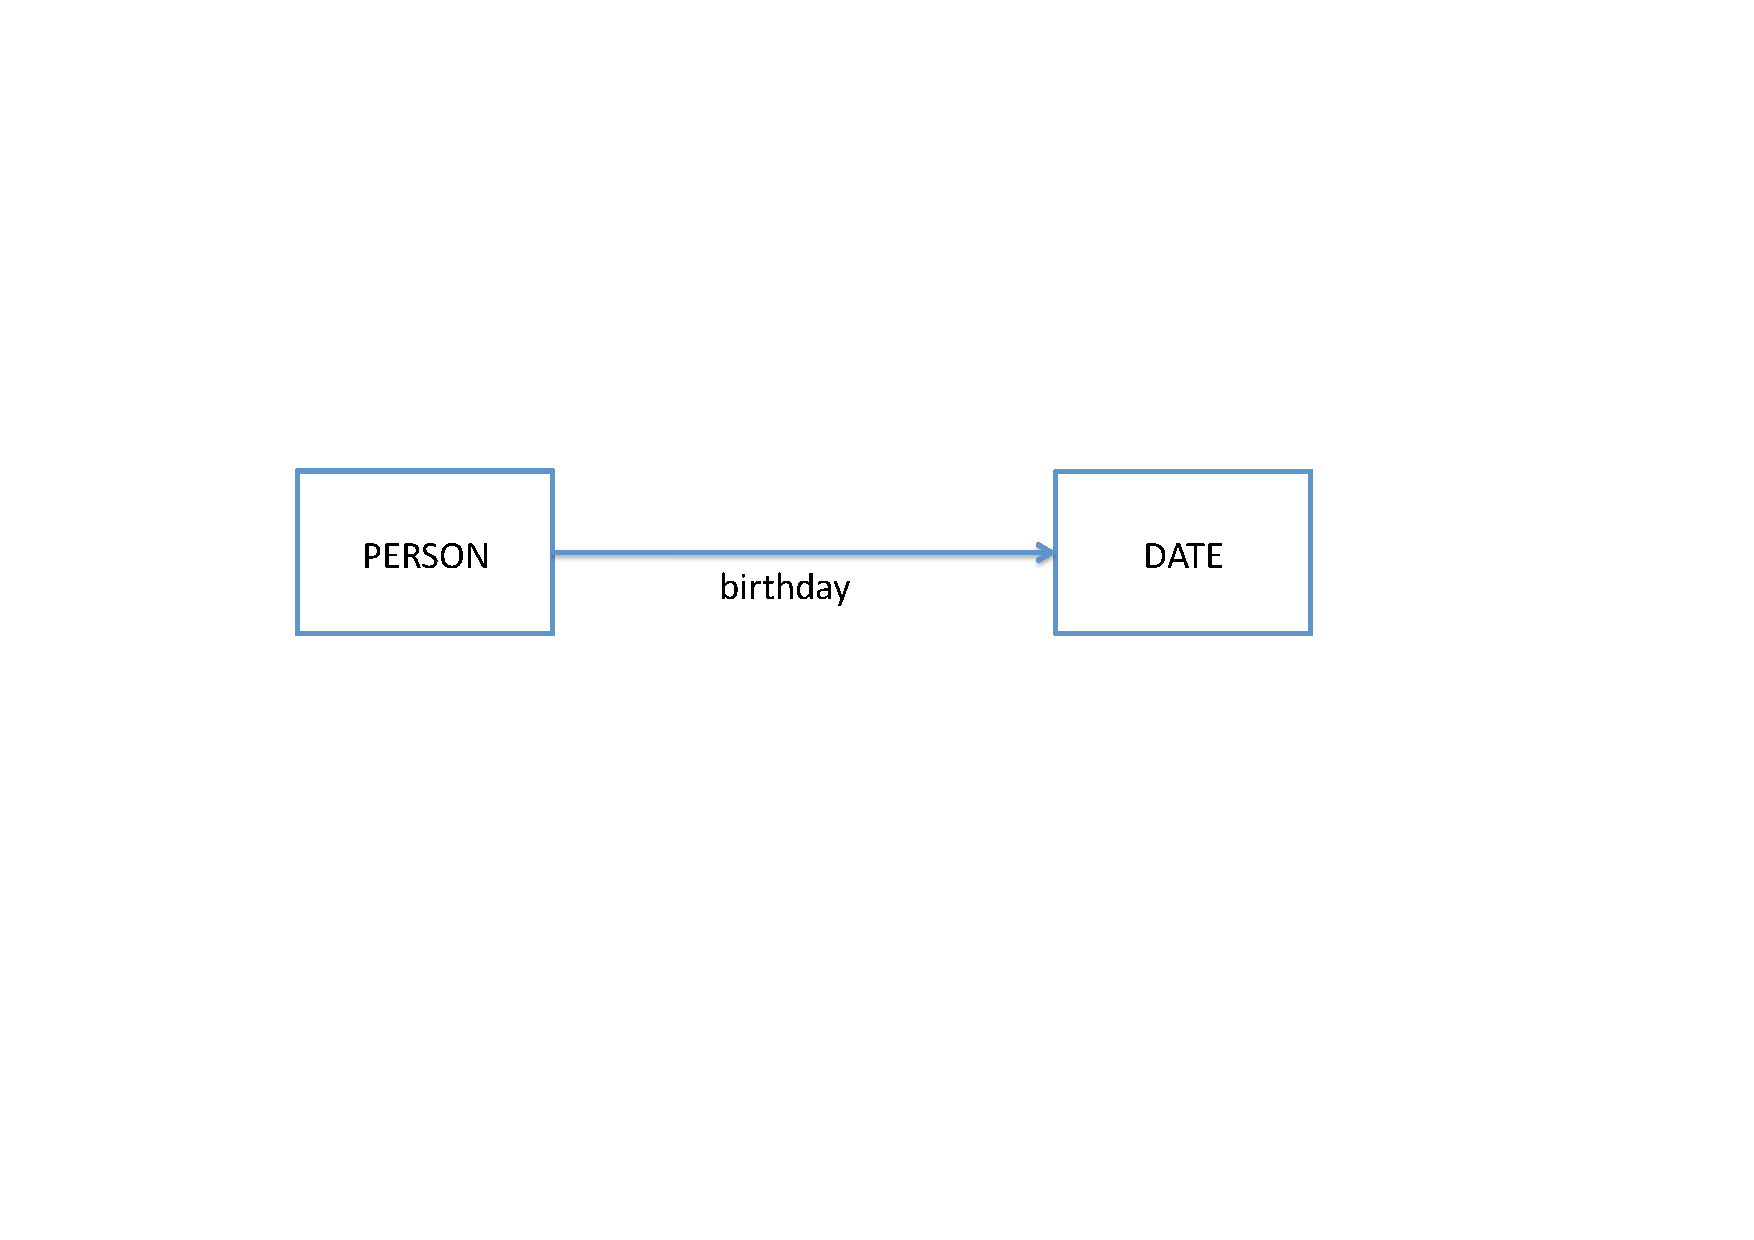
\includegraphics[scale=.5]{bb1}
  \end{center}

\end{frame}




\begin{frame} \frametitle{Making variable set explicit}

  \begin{center}
    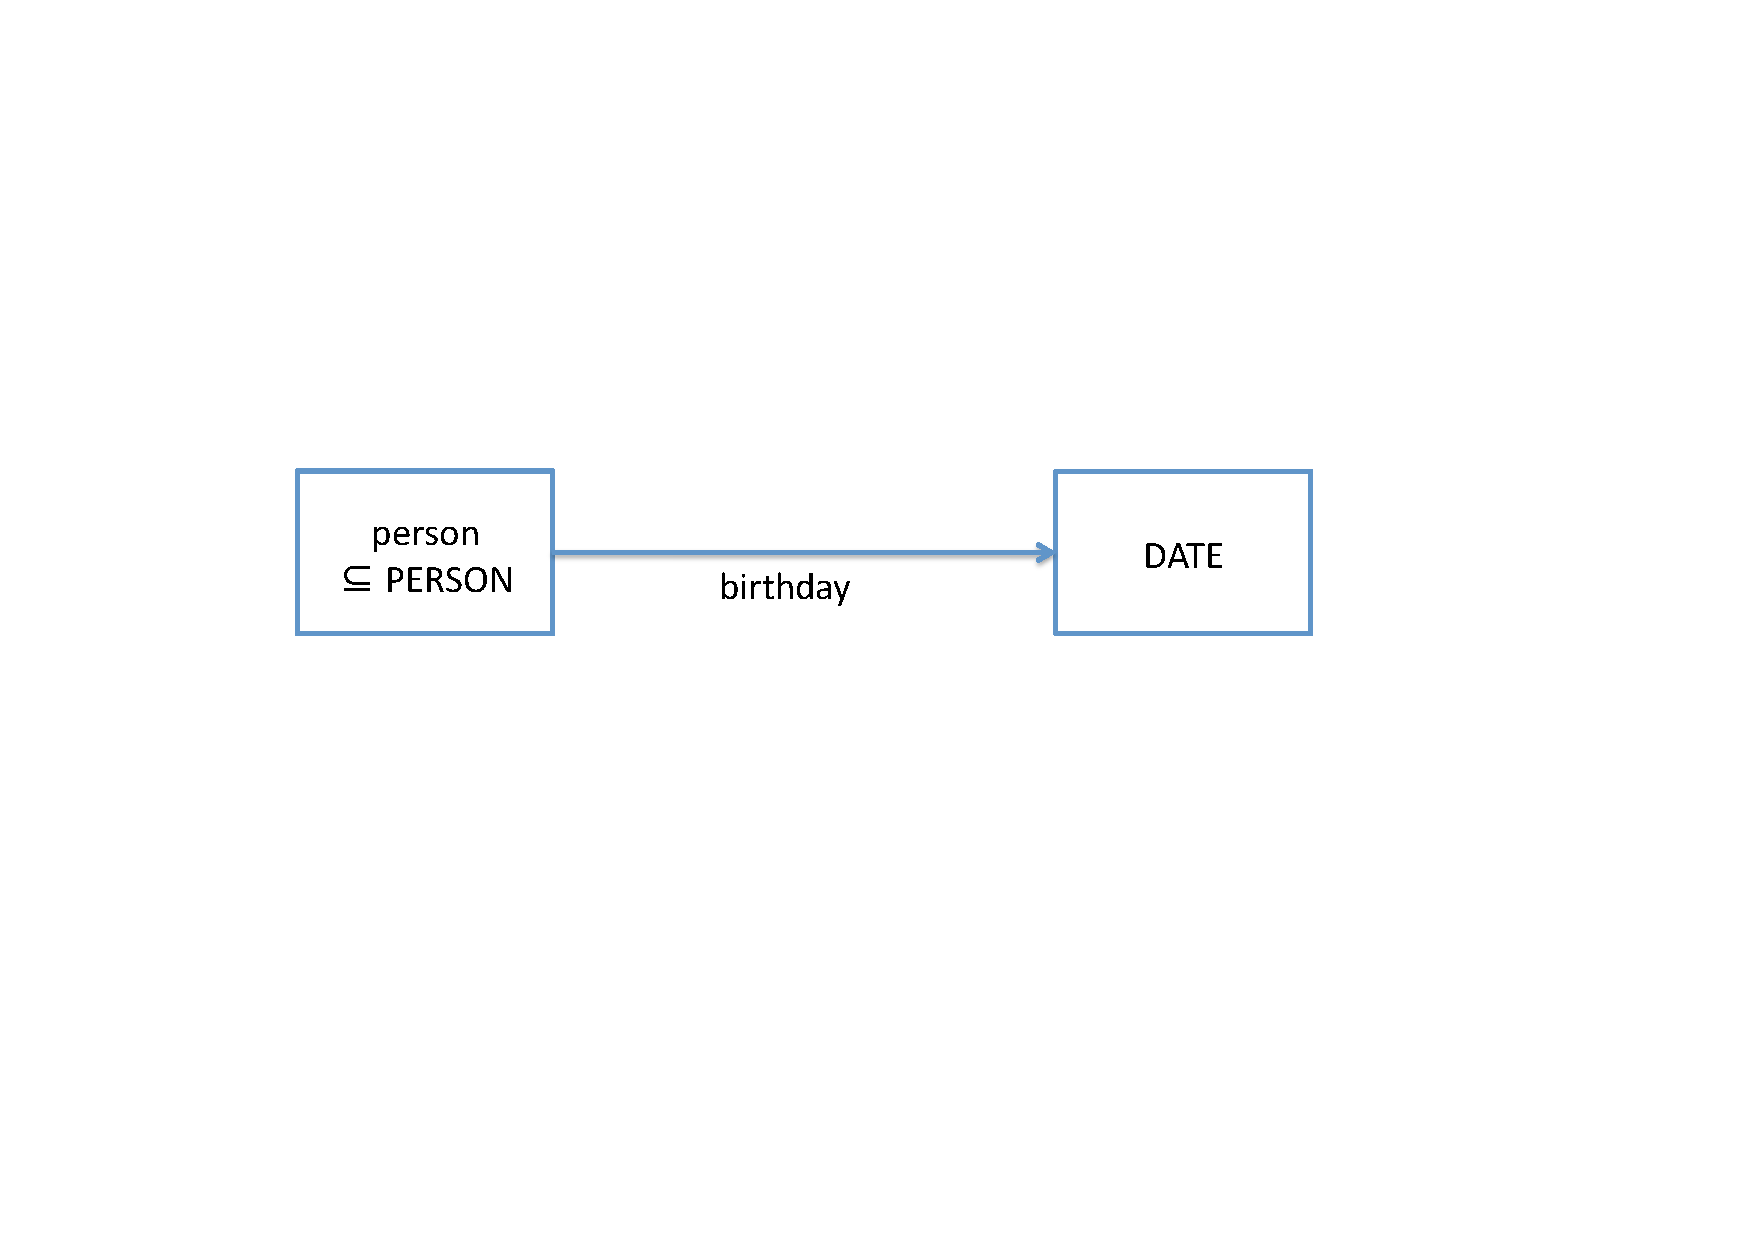
\includegraphics[scale=.5]{bb2}
  \end{center}

\end{frame}



\begin{frame}

\frametitle{Secure database example}



We consider a  secure database. Each object in the database has a
 odata component.

~

Each object has a classification between 1 and 10.

~

Users of the system have a clearance level between 1 and 10.

~

Users can only read and write objects whose classification is no
greater than the user's clearance level.

~

What are the \textit{types, variables, events}?





\end{frame}






\begin{frame} \frametitle{Class diagram}

  \begin{center}
    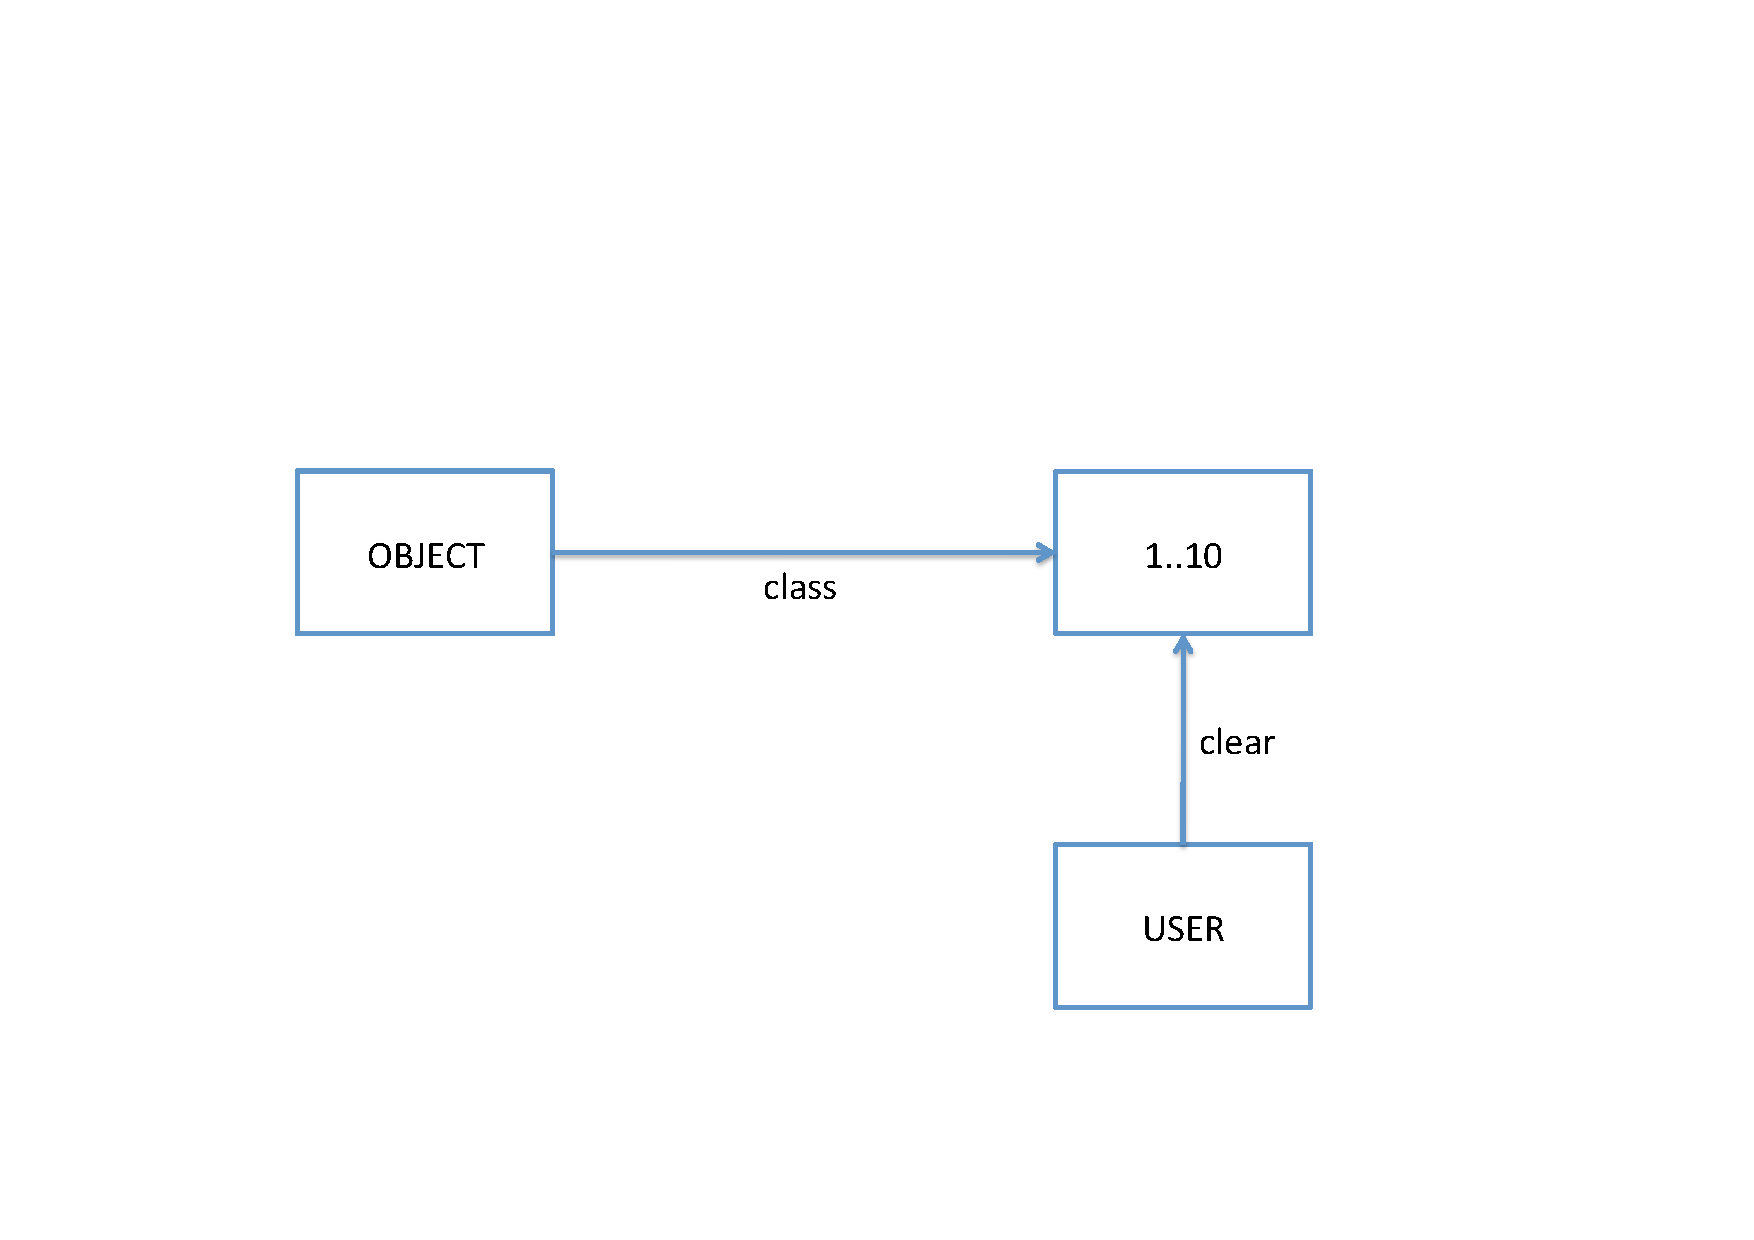
\includegraphics[scale=.5]{sdb4}
  \end{center}

\end{frame}




\begin{frame} \frametitle{Class diagram}

  \begin{center}
    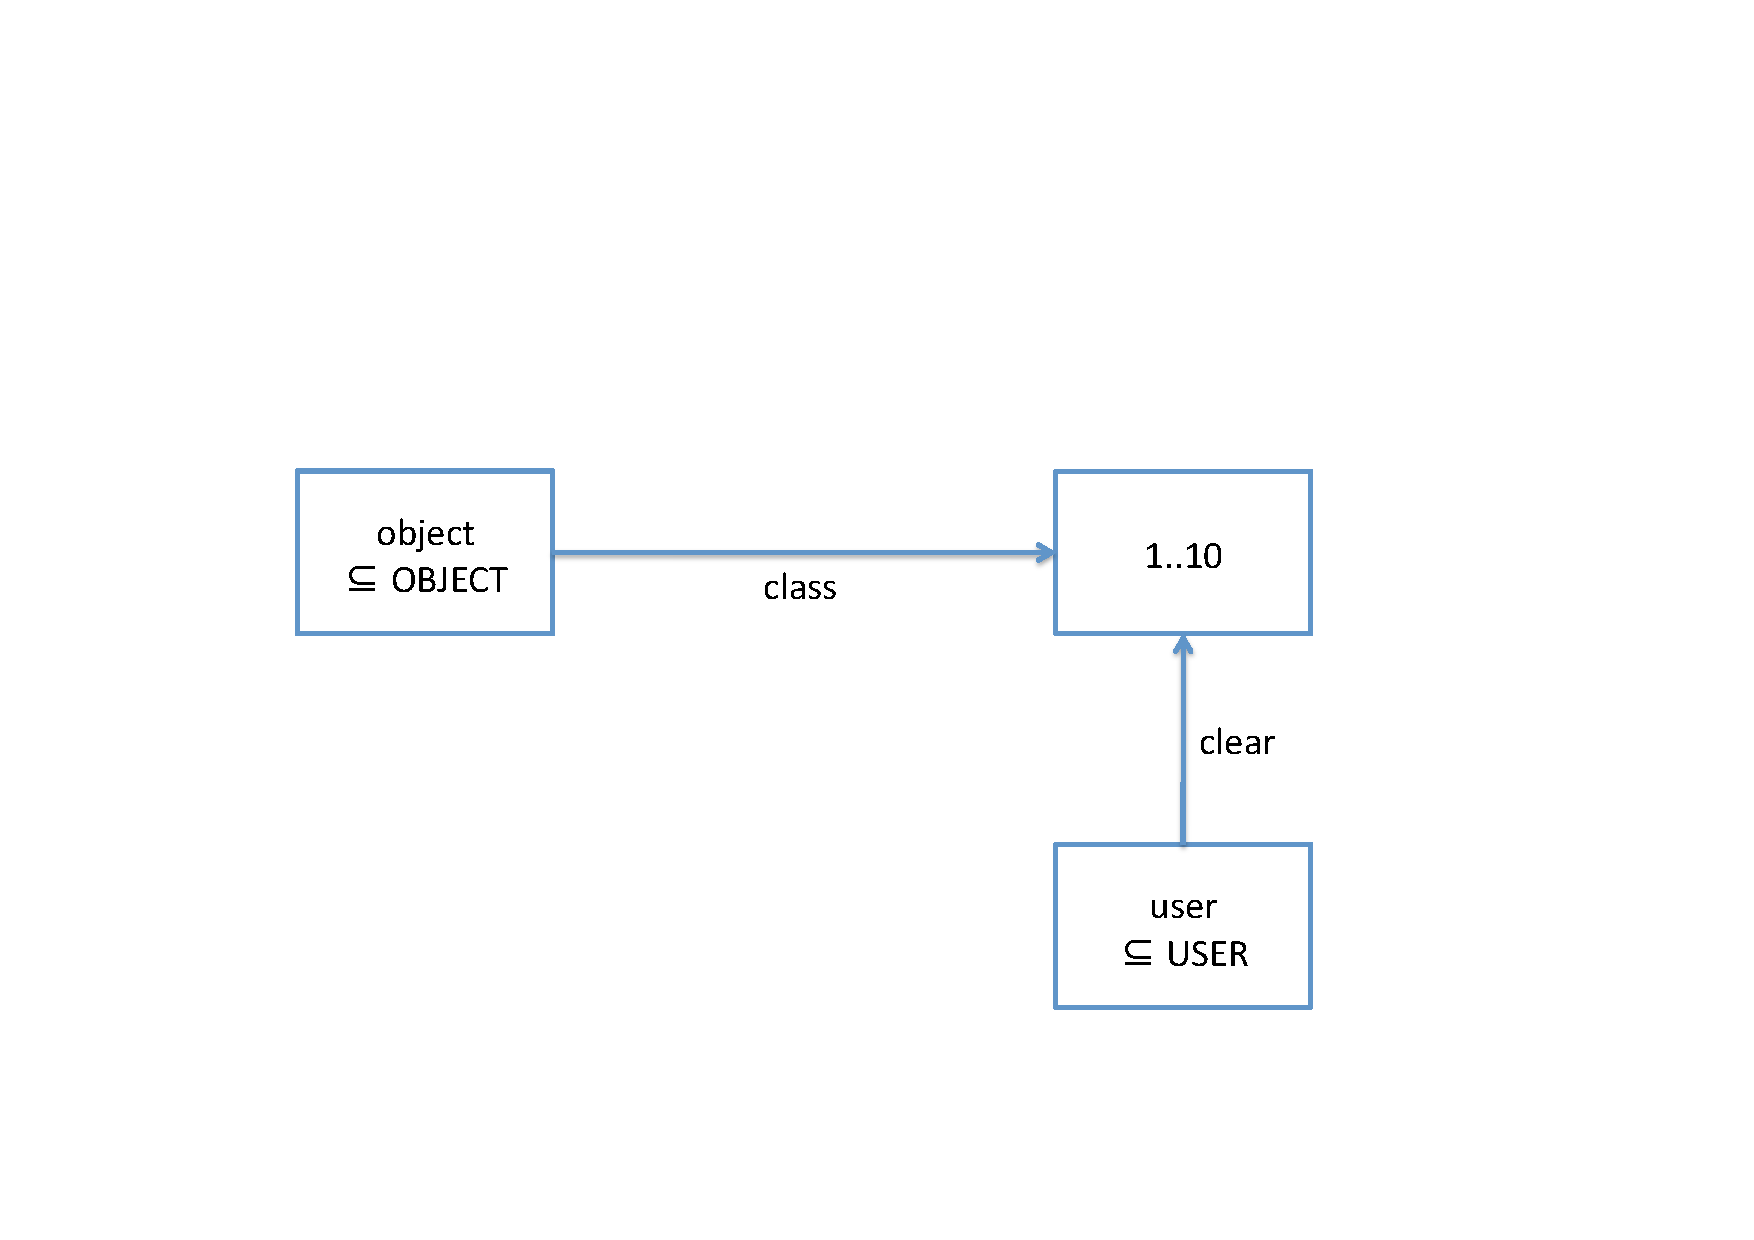
\includegraphics[scale=.5]{sdb5}
  \end{center}

\end{frame}




\begin{frame}
\frametitle{Types and variables}


\setsA{
     OBJECT ~~~    USER
}
%
\variablesA{object,~ user,~  class,~ clear}
%
\pause
\invariant{
    object ~\subseteq~ OBJECT ~\\
    user ~\subseteq~ USER ~\\
        class ~\in~ object \tfun (1..10) ~\\
        clear ~\in~ user \tfun (1..10)
          }

~

\initialisationA{
   object:=\set{}~~~~ user:=\set{}~~~~ class:=\set{}~~~~ clear:=\set{} }

\end{frame}




\begin{frame} \frametitle{Class diagram for secure database}

  \begin{center}
    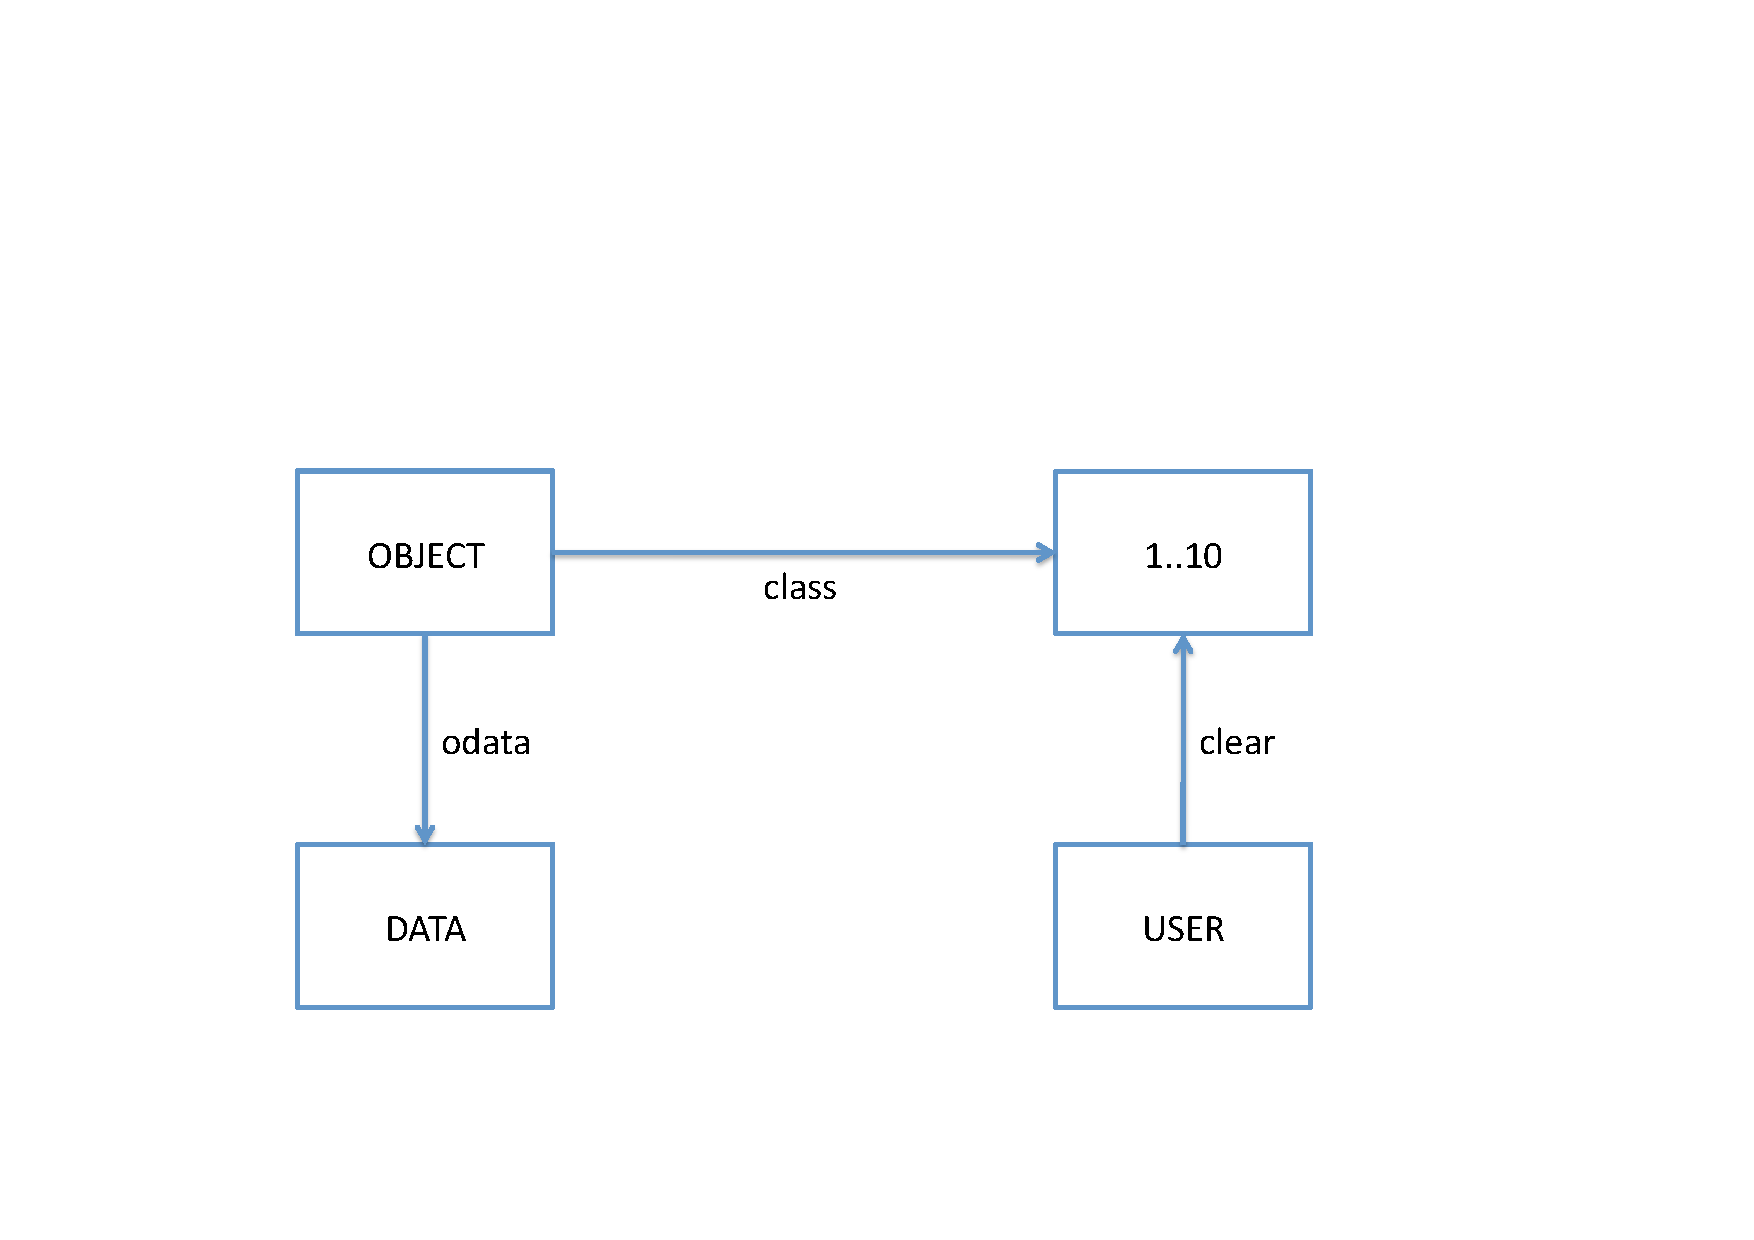
\includegraphics[scale=.5]{sdb1}
  \end{center}

\end{frame}





\begin{frame} \frametitle{Making variable set explicit}

  \begin{center}
    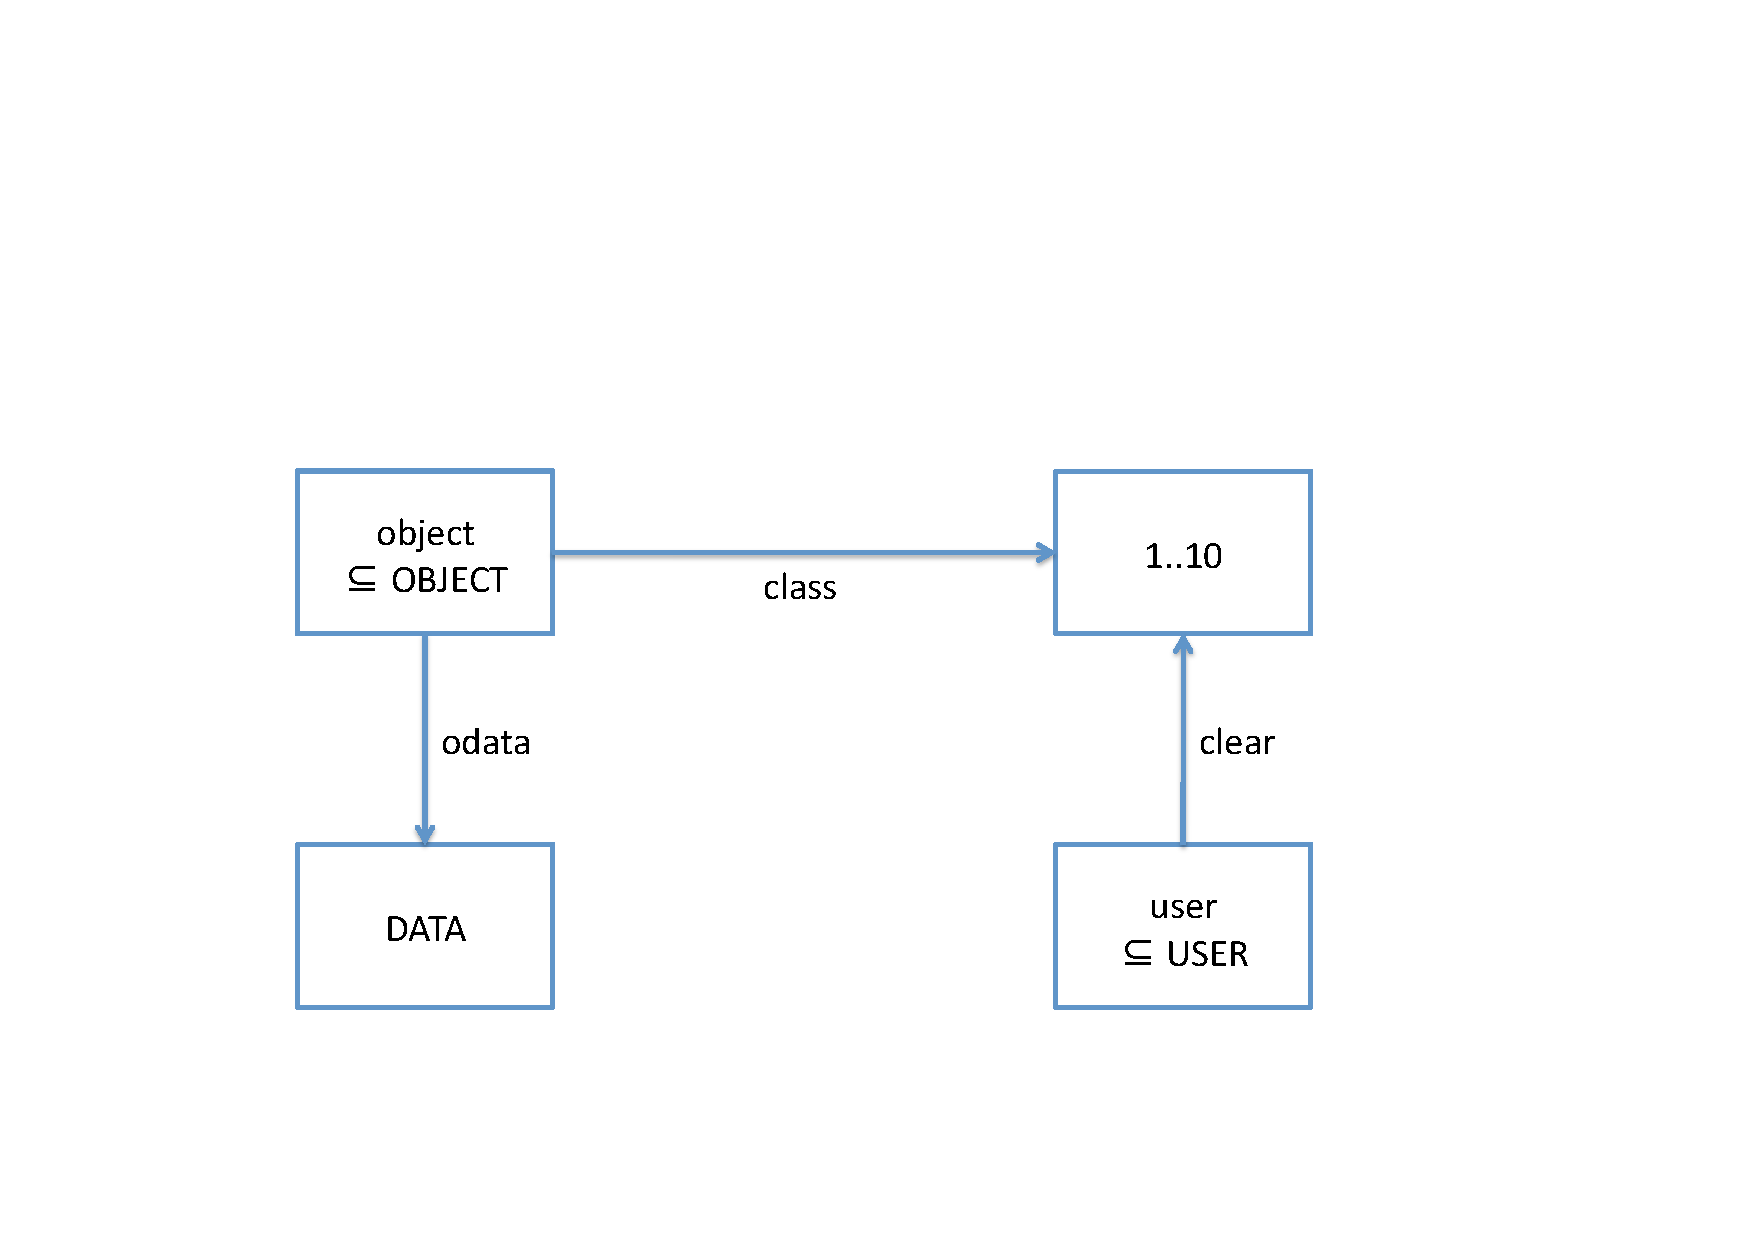
\includegraphics[scale=.5]{sdb2}
  \end{center}

\end{frame}





\begin{frame}
\frametitle{Types and variables}


\setsA{
     OBJECT ~~~  DATA ~~~ USER
}
%
\variablesA{object,~ user,~ odata,~ class,~ clear}
%

\invariant{
    object ~\subseteq~ OBJECT ~\\
    user ~\subseteq~ USER ~\\
       odata ~\in~ object \tfun DATA ~\\
        class ~\in~ object \tfun (1..10) ~\\
        clear ~\in~ user \tfun (1..10)
          }

The \alert{invariant} $odata ~\in~ object \tfun DATA$  means that $odata(o)$ is
well-defined whenever $o\in object$.  ~~ Why is this important?

~

\initialisation{
    object:=\set{}~~~~ user:=\set{}
~~~~odata:=\set{}~~~~ class:=\set{}~~~~ clear:=\set{} }

\end{frame}





\begin{frame}

\frametitle{Adding users}

 \operB{AddUser}{
 \pause
    \anyB{u,c}{
         u ~\in~ USER ~~\\
       u ~\not\in~ user ~~\\
        c ~\in~ 1..10
    }{
        user ~\assign~ user \cup \set{u} \\
        clear(u) ~\assign~ c
    } }

The new user must not already exist.

We need to provide the initial clearance level for the new user.
\end{frame}




\begin{frame}

\frametitle{Adding objects}

\operB{AddObject}{
\pause
    \anyB{o,d,c}{
        o ~\in~ OBJECT  ~~ \\
        o ~\not\in~  object ~~ \\
        d ~\in~ DATA ~\\
		c ~\in~ 1..10
    }{
        object ~\assign~ object \cup \set{o}  \\
        odata(o) ~\assign~ d  \\
        class(o) ~\assign~ c
    } }

The new object must not already exist.

We need to provide the initial classification level and odata value
for the new object.

\end{frame}




\begin{frame}

\frametitle{Reading objects}

 \operB{Read}{
 \pause
    \anyBs{u,o,d!}{ \begin{array}{ll}
        u ~\in~ user ~~  & \mbox{The user must exist} \\
        o~\in~ object ~~ & \mbox{The object must exist}\\
        clear(u) \geq class(o)~~~~  & \mbox{The clearance must be ok} \\
        d! = odata(o)  & \mbox{The odata associated with the object}
           \end{array}
    } }

\end{frame}




\begin{frame}
\frametitle{Writing objects}

 \operB{Write}{
 \pause
    \anyB{u,o,d}{
        u ~\in~ user ~~ \\
        o~\in~ object ~~\\
        clear(u) \geq class(o)
    }{
        odata(o) ~\assign~ d
    } }

    The write operation overwrites the odata value associate with
    the object with a new value.
\end{frame}




\begin{frame}
\frametitle{Changing classification and clearance levels}

\begin{columns}
\begin{column}{2in}
\operB{ChangeClass}{
    \anyB{o,c}{
                o ~\in~ object ~~\\
                c ~\in~ 1..10
    }{
        class(o) ~\assign~ c
    } }
\end{column}
\begin{column}{2in}
 \operB{ChangeClear}{
    \anyB{u,c}{
                u ~\in~ user ~~\\
                c ~\in~ 1..10
    }{
        clear(u) ~\assign~ c
    } }
\end{column}
\end{columns}



\end{frame}




\begin{frame}

\frametitle{Removing users and objects}

\begin{columns}
\begin{column}{2in}
 \operB{RemoveUser}{
 \pause
    \anyB{u}{
        u ~\in~ user
    }{
        user ~\assign~ user \setminus \set{u}  \\
        clear := \set{u} \domsub clear
    } }
\end{column}
\begin{column}{2in}
\pause
 \operB{RemoveObject}{
 \pause
    \anyB{o}{
        o ~\in~ object
    }{
        object ~\assign~ object \setminus \set{o}  \\
        class := \set{o} \domsub class \\
        odata := \set{o} \domsub odata
    } }
\end{column}
\end{columns}


\end{frame}





\begin{frame}

\frametitle{Adding object ownership}

Extend the database specification so that each object has an owner.

~

The clearance associated with that owner must be at least as
high as the classification of the object.  

~

Only the owner of an
object is allowed to delete it.

~

A user's clearance level can only be modified to a new level 
by another user whose clearance level is at least as high as the 
new clearance level.

~

What additional variables are required?

~

What events are affected?





\end{frame}


\begin{frame} \frametitle{Class diagram with ownership}

  \begin{center}
    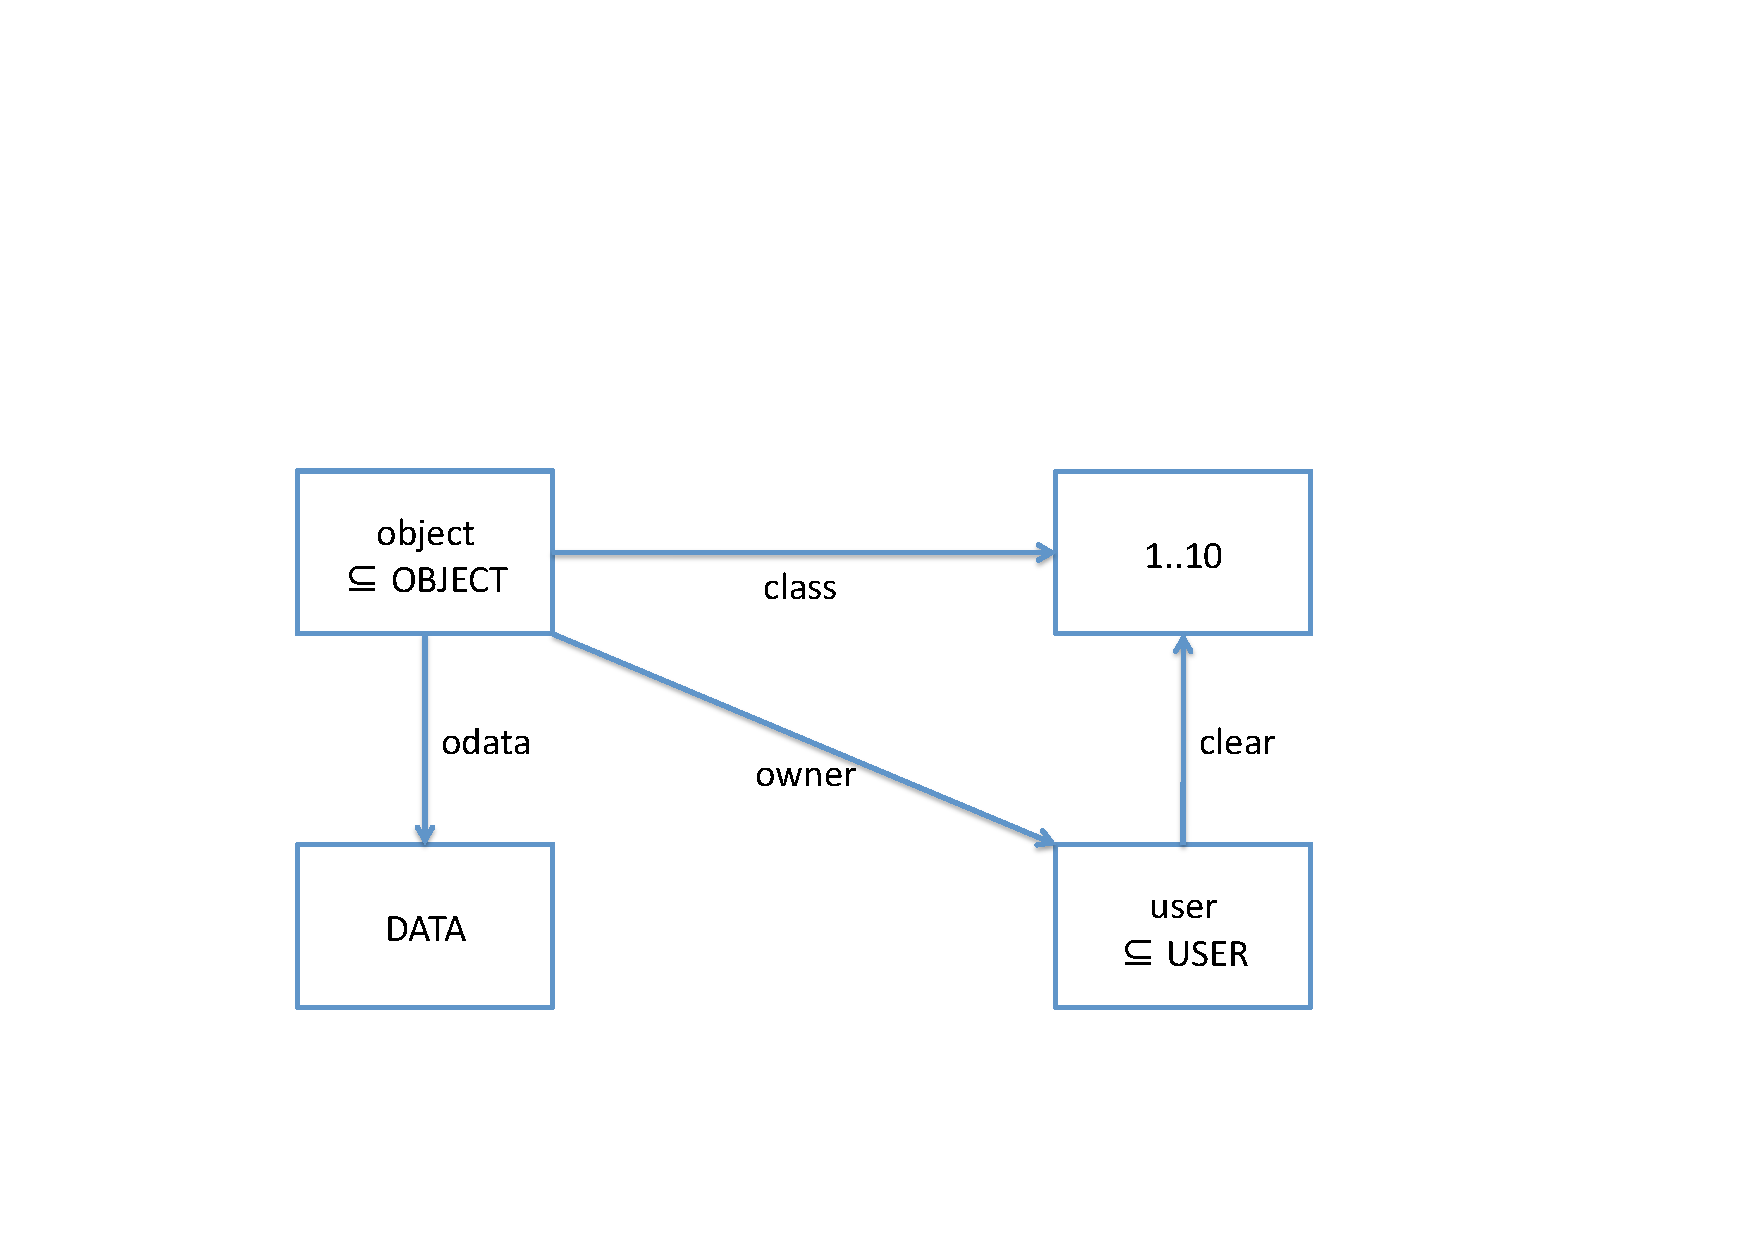
\includegraphics[scale=.5]{sdb3}
  \end{center}

\end{frame}




\end{document}




\begin{frame}

\frametitle{Nondeterministic actions}
Assign a value from set $S$ to variable $x$:~~~~
\fbox{$
~x~:\in~S~
$}

~~~~Feasibility obligation: $S$ is non-empty.

Assign a value satisfying $P$ to variable $x$:~~~~
\fbox{$
~x~:\!|~~ P(x,x')~
$}

~~~~Example, increase x:~~~  $x~ :\!|~~ x'>x$

~~~~Feasibility obligation: $P$ is satisfiable:~~~~  $\exists x'.P$

\end{frame}




\begin{frame}

\frametitle{Implicit Specification}
{Find the position of a value in an array:}

\variablesA{array,k}
\invariantA{array\in (1..N) \tfun T ~~\land~~ k\in(1..N)}

 \operB{FindPosition}{
    \anyB{t}{ t ~\in~ T }{\mbox{Set k so that $array(k)=t$}}
}

\end{frame}






\begin{frame}


\frametitle{Find the position of a value in an array}

\variablesA{array,k}
\invariantA{array\in (1..N) \tfun T ~~\land~~ k\in(1..N)}


 \operB{FindPositionOK}{
    \anyB{t,k'}{ t ~\in~ T \\
    k' ~\in~ 1..N \\
    array(k')=t  }{ k := k' }
}

What if $t\not\in ran(array)$~ ?


\end{frame}




\begin{frame}


\frametitle{Explicit guarding}


\begin{minipage}[t]{5in}
 \operB{FindPositionOK}{
    \anyB{t,k'}{ t ~\in~ ran(array) \\
    k' ~\in~ 1..N \\
    array(k')=t  }{ k := k' }
}
\end{minipage}
\begin{minipage}[t]{4in}

 \operB{FindPositionKO}{
    \anyB{t}{ t ~\not\in~ ran(array) }{k:=0}
}
\end{minipage}



\end{frame}




\begin{frame}


\frametitle{Find the first occurrence}

\operB{FindPositionOK}{
    \anyB{t,k'}{ t ~\in~ ran(array) \\
    k' ~\in~ 1..N \\
    array(k')=t\\
    \forall j \cdot j\in 1..N ~\land~ array(j)=t ~~\implies~~ k'\leq j
      }{ k := k' }
}


\end{frame}




\begin{frame}


\frametitle{Find the first occurrence, alternative formulation}
%
\operB{FindPositionOK}{
    \anyB{t,k'}{ t ~\in~ ran(array) \\
    k' = min(dom(array\ranres\set{t}))
      }{ k := k' }
}
%
\operB{FindPositionOK}{
    \anyB{t}{ t ~\in~ ran(array)
      }{ k := min(dom(array\ranres\set{t})) }
}




\end{frame}





\begin{frame}

\frametitle{Sort an array}

\variablesA{array}
\invariantA{array\in (1..N) \tfun \nat }

 \operB{Sort}{
    \anyB{array'}{ array' ~\mbox{is sorted} }{array:=array'}
}

\end{frame}



\begin{frame}


\variablesA{array}
\invariantA{array\in (1..N) \tfun \nat }

 \operB{Sort}{
    \anyB{array'}{%
    \forall i \cdot i\in 1..N-1 ~~\implies~~ array'(i) \leq array'(i+1) }{ %
    array:=array'}
}

Is this enough?


\end{frame}





\begin{frame}

\frametitle{Permutation}


 \operB{Sort}{
    \anyB{array'}{%
    \forall i \cdot i\in 1..N-1 ~~\implies~~ array'(i) \leq array'(i+1) \\
    \forall x \cdot x\in \nat ~~\implies~~ card(array'\ranres\set{x}) = card(array\ranres\set{x}) }{ %
    array:=array'}
}



\end{frame}









\end{document}



